\documentclass[11pt]{beamer}
%\usepackage{multicol}
\usepackage[vietnamese]{babel}
\usefonttheme[onlymath]{serif}
\usepackage{tgbonum}%chagne font

\usetheme[progressbar=frametitle]{metropolis}
\setbeamertemplate{frame numbering}[fraction]
\useoutertheme{metropolis}
\useinnertheme{metropolis}
\usefonttheme{metropolis}
\usecolortheme{spruce}
\setbeamercolor{background canvas}{bg=white}

\definecolor{mygreen}{rgb}{.125,.5,.25}
\usecolortheme[named=mygreen]{structure}

\usepackage{ragged2e}
\apptocmd{\frame}{}{\justifying}{}

\usepackage{graphicx,environ}
\usepackage{hyperref}

\NewEnviron{sourcefigure}[1][htbp]{%
	{\let\caption\relax\let\ref\relax
		\renewcommand{\label}[1]{%
			\gdef\sfname{sf:##1}}%
		\setbox1=\hbox{\BODY}}% Capture \label
	\global\expandafter\let\csname\sfname\endcsname\BODY% Capture entire figure
	\begin{figure}[#1]
		\BODY
	\end{figure}
}
\newcommand{\reusefigure}[2][htbp]{%
	{\addtocounter{figure}{-1}%
		\renewcommand{\theHfigure}{dupe-fig}% If you're using hyperref
		\renewcommand{\thefigure}{\ref{#2}}% Figure counter is \ref
		%\renewcommand{\thefigure}{\ref{#2} (repeated)}% Figure counter + "(repeated)"
		\renewcommand{\addcontentsline}[3]{}% Avoid placing figure in LoF
		\renewcommand{\label}[1]{}% Make \label inactive
		\begin{figure}[#1] \csname sf:#2\endcsname \end{figure}}
}

\usepackage{array}
\usepackage{booktabs}

\usepackage{subcaption}
\setbeamertemplate{caption}[numbered] 

\title{Điều khiển PLL kỹ thuật số cho hệ thống quang điện một pha}
%\subtitle{Subtitle Here}
\author{Lê Thanh Hải - 20191813\\GVHD: TS. Trần Thanh Sơn\\[20pt]}
%\institute{\large \textbf{Learning Outcomes}: \\[6pt] Identify properties of elementary functions (formed by composition of power, exponential, logarithmic, and trigonometric functions and their inverses).}
\date{\today}

\makeatletter
\setbeamertemplate{title page}{
	\begin{minipage}[b][\paperheight]{\textwidth}
		\centering  % <-- Center here
		\ifx\inserttitlegraphic\@empty\else\usebeamertemplate*{title graphic}\fi
		\vfill%
		\ifx\inserttitle\@empty\else\usebeamertemplate*{title}\fi
		\ifx\insertsubtitle\@empty\else\usebeamertemplate*{subtitle}\fi
		\usebeamertemplate*{title separator}
		\ifx\beamer@shortauthor\@empty\else\usebeamertemplate*{author}\fi
		\ifx\insertdate\@empty\else\usebeamertemplate*{date}\fi
		\ifx\insertinstitute\@empty\else\usebeamertemplate*{institute}\fi
		\vfill
		\vspace*{1mm}
	\end{minipage}
}

\setbeamertemplate{title}{
	%  \raggedright%  % <-- Comment here
	\linespread{1.0}%
	\inserttitle%
	\par%
	\vspace*{0.5em}
}
\setbeamertemplate{subtitle}{
	%  \raggedright%  % <-- Comment here
	\insertsubtitle%
	\par%
	\vspace*{0.5em}
}
\makeatother

%\setbeamercovered{transparent=5}

\begin{document}
	\metroset{block=fill}

% Slide 1	
	\begin{frame}
		\titlepage
	\end{frame}



% Slide 2
	\begin{frame}[t]{Thông tin bài báo khoa học} \vspace{4pt}
		\begin{columns}
			
			\begin{column}{0.5\textwidth}
				%\vspace{4pt}
				\textbf{Tác giả}: Jong-Woo Choi, Young-Jun Kim, Hwangnam Kim
				
				\vspace{4pt}
				\textbf{DOI}: 10.1049/ip-epa:20045225
				
				\vspace{7pt}
				\emph{IEE Proc.-Electr. Power Appl.}, Vol. 153, No. 1, January 2006
				
			\end{column}
		
			\begin{column}{0.5\textwidth}  %%<--- here
				\begin{center}
					%\vspace{1in}
					\begin{figure}[h]
						\textbf{Scan QR-Code}
						
\includegraphics[width=1\textwidth]{QRCode.jpg}
						%\label{fig:QR-Code}
					\end{figure}
				\end{center}
			\end{column}
		\end{columns}
		Các tác giả đến từ Trường Kỹ thuật Điện-Điện tử,~Kyungpook, Đại học Quốc gia, Sangyeok-dong, Buk-gu, Daegu, Hàn Quốc.
	\end{frame}


% Slide 3
	\begin{frame}[t]{NỘI DUNG} \vspace{4pt}
		\Large{\tableofcontents}
		
	\end{frame}


\section{1 Giới thiệu}
% Slide 4
	\begin{frame}[t]{1 Giới thiệu}	
		
		Thông tin điện áp lưới, chẳng hạn như tần số, góc pha và biên độ, rất quan trọng trong nhiều hệ thống công nghiệp.
		
		Trong hệ thống ba pha, thông tin về điện áp lưới có thể dễ dàng thu được bằng cách sử dụng phương pháp vecto.
		
		Tuy nhiên, đối với hệ thống một pha, thông tin điện áp khó có được hơn nhiều.
		
		Thông thường, tần số và góc pha của điện áp một pha thu được bằng cách “bắt điểm qua không”.
		
		Tuy nhiên, phương pháp này không thể cung cấp thông tin điện áp lưới ngay lập tức và rất nhạy cảm với nhiễu.
			
		
	\end{frame}

% Slide 5
	\begin{frame}[t]{1 Giới thiệu}		
		Theo đó, bài báo trình bày một thuật toán vòng khóa pha kỹ thuật số (PLL) mới cho các hệ thống quang điện một pha. 
		
		Thuật toán sử dụng hai giai đoạn ảo và hiệu suất của nó được chứng minh trong các điều kiện khác nhau để cho thấy tính hiệu quả của thuật toán được đề xuất. 
		
	\end{frame}

\section{2 Phương pháp bắt điểm qua không}
% Slide 6
	\begin{frame}[t]{2 Phương pháp bắt điểm qua không}
		Hình~\ref{fig:Zero-cross-detection method} cho thấy phương pháp bắt điểm qua không, trong đó điểm không được phát hiện sau mỗi nửa chu kỳ. Góc ước lượng $\hat{\theta}$ thu được bằng cách tích phân tần số ước tính $\hat{\omega}$, tần số này được ước tính bằng cách điều khiển chênh lệch góc về 0 trong bộ điều khiển PI. Trong hình~\ref{fig:Zero-cross-detection method}, $\omega_{set}$ là giá trị tần số ban đầu.
		
		% Fig 1
		\begin{figure}[h]
			 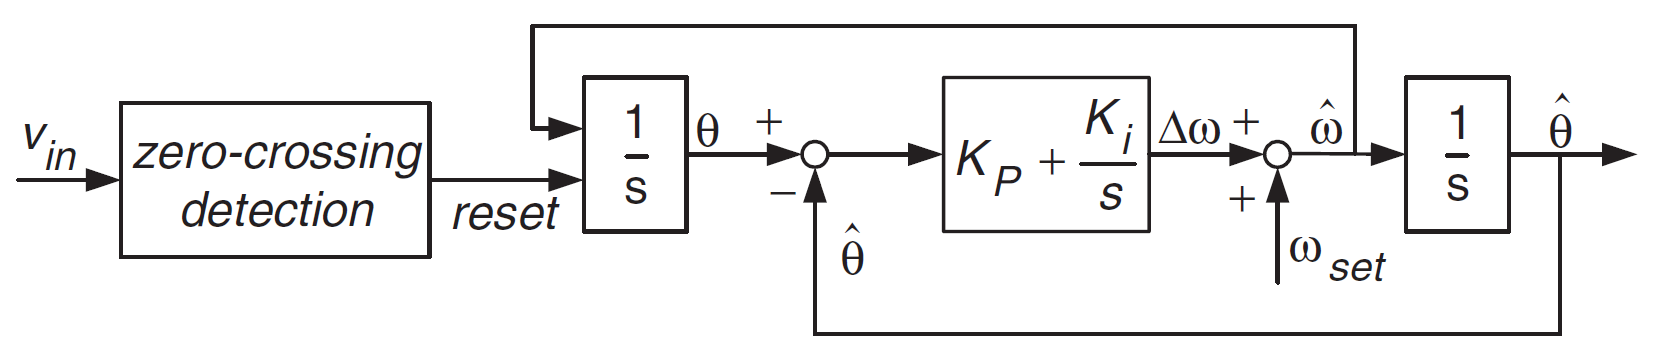
\includegraphics[width=1\textwidth]{Fig. 1 Zero-cross-detection method.PNG}  
			 \caption{\textit{Phương pháp bắt điểm qua không}}
			 \label{fig:Zero-cross-detection method}
		 \end{figure} 
		
	\end{frame}

% Slide 7
	\begin{frame}[t]{2 Phương pháp bắt điểm qua không}
		\begin{columns}
			
			\begin{column}{0.5\textwidth}
				%\vspace{5pt}
				\justifying
				\vspace{5pt}
				
				Hình~\ref{fig:Lưu đồ phương pháp bắt điểm qua không} cho thấy một sơ đồ khối của phương pháp bắt điểm qua không, trong đó giá trị ở thời điểm hiện tại được lấy mẫu cho điện áp lưới được nhân với khoảng thời gian được lấy mẫu trong quá khứ, cho phép phát hiện điểm giao nhau.
				\vspace{0.8cm}
				
				Nếu giá trị hiện tại lớn hơn 0 thì góc pha $\theta$ bằng 0; ngược lại, góc pha $\theta$ là $\pi$.
				
			\end{column}
			
			\begin{column}{0.5\textwidth}  %%<--- here
				\begin{center}
					%\vspace{1in}
					
					\begin{figure}[h]
						%\textbf{Scan QR-Code}
						%\caption{\textit{Flowchart of zero-cross-detection method}}
						%\label{fig:Flowchart of zero-cross-detection method}
						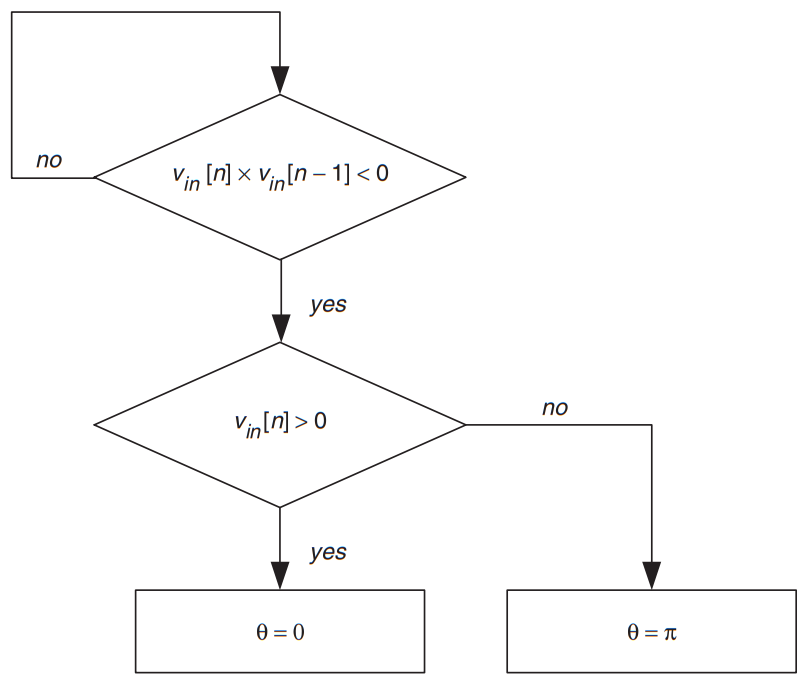
\includegraphics[width=1\textwidth]{Fig. 2 Flowchart of zero-cross-detection method}
						\caption{\centering \textit{Lưu đồ phương pháp bắt điểm qua không}}
						\label{fig:Lưu đồ phương pháp bắt điểm qua không}
					\end{figure}	
				\end{center}
			\end{column}			
		\end{columns}
	\end{frame}

% Slide 8
	\begin{frame}[t]{2 Phương pháp bắt điểm qua không}
		%\vspace{4pt}
		
		Tuy nhiên, khuyết điểm của phương pháp này là độ nhạy của nó đối với nhiễu.
		\vspace{0.1cm}
		
		Nếu nhiễu tác động vào điện áp lưới, một lỗi phát hiện pha xảy ra, vì điểm không sẽ được phát hiện nhiều lần.
		
	\end{frame}


\section{3 Phân tích bộ Dò hai pha ảo}
% Slide 9
	\begin{frame}[t]{3 Phân tích bộ Dò hai pha ảo}
		%\vspace{4pt}
		
		Bộ dò pha được chia thành hai phần:
		\begin{itemize}
			\item \textbf{Bộ tạo hai pha ảo}: Tạo ra $V_d^s$ và $V_q^s$ vuông pha nhau.
			\item \textbf{Bộ điều khiển pha}: Điều chỉnh $V_d^s$ và $V_q^s$ để tạo ra góc pha ước tính $\hat\theta$, tần số ước tính $\hat{\omega}$ và biên độ ước tính $\hat{E}$.
		\end{itemize}
	
		\begin{sourcefigure}[h]
			
			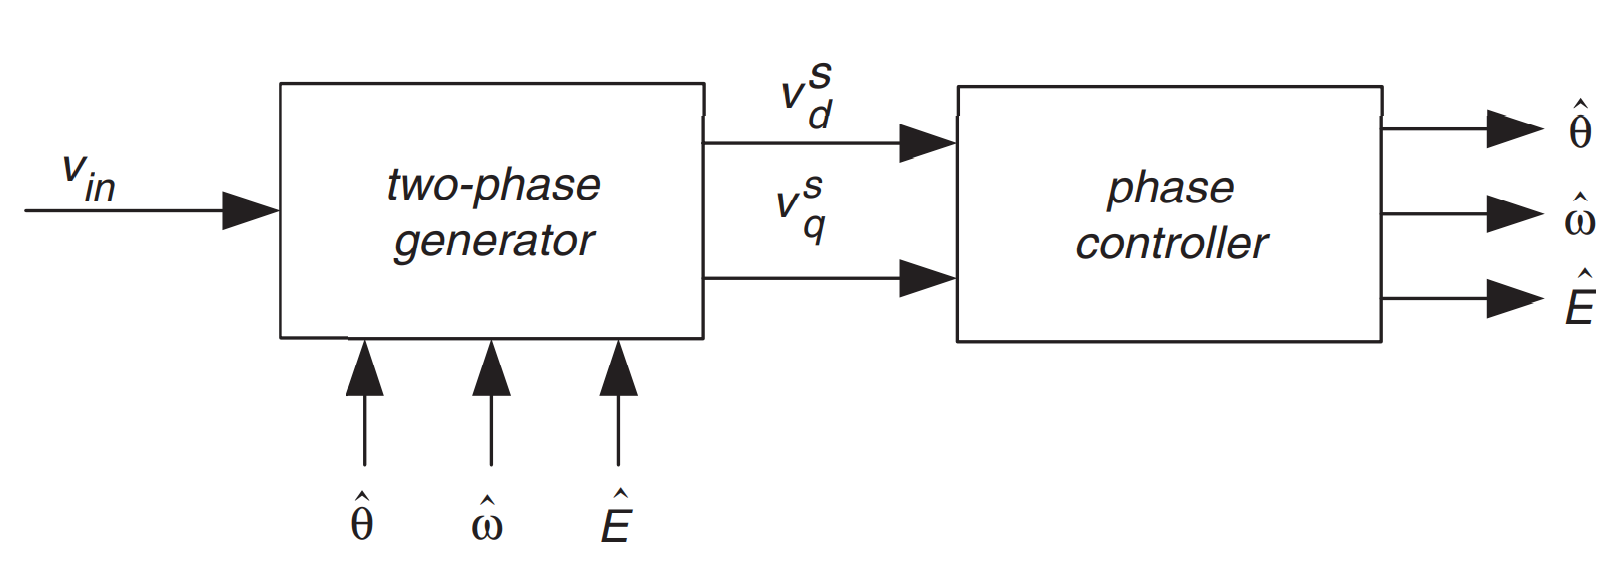
\includegraphics[width=1\textwidth]{Fig. 3 Virtual two-phase detector.PNG}
			\caption{\textit{Bộ Dò 2 pha ảo}}
			\label{fig:Bộ Dò 2 pha ảo}
		\end{sourcefigure}
		
		
	\end{frame}

% Slide 10
%\subsection{3.1 Two-phase Generator}
\begin{frame}[t]{3.1 Bộ tạo hai pha ảo}
	%\vspace{4pt}
	
	Biểu thức điện áp đầu vào trong hình~\ref{fig:Bộ Dò 2 pha ảo}:
	$$v_{in}=E\sin({\omega t})=E\sin({\theta})$$
	Hai đầu ra của bộ tạo hai pha ảo:
	\begin{align*}
		{v}_q^s &=E\sin({\omega t})=v_{in}\\
		v_d^s &=E\cos({\omega t})
	\end{align*}

	%{\fontfamily{CM Roman}\selectfont
	%	This text uses a different font $v=b$ typeface
	%}

	%$$v_d^s =E\sin({\omega t})=v_{in}$$
	%$$v_q^s =E\cos({\omega t})$$
	
	
\end{frame}

% Slide 11
	\begin{frame}[t]{(a) Phương pháp sử dụng bảng bộ nhớ}
				
				$v_{in}$ được lưu giữ vào bộ nhớ mỗi chu kỳ và				
				%$$v_q^s = v_{in}$$
				giá trị của $v_{in}$ ở $1/4$ chu kỳ trước sẽ được nhân với $-1$
				%$$v_d^s=-v_{in} \left( t-\frac{\pi}{2 \hat{\omega}} \right)=-E \sin{\left( \omega t-\frac{\omega}{\hat{\omega}} \frac{\pi}{2}  \right)} \cong E \cos{\omega t} $$
				\begin{align*}
					v_d^s&=-v_{in} \left( t-\frac{\pi}{2 \hat{\omega}} \right)=-E \sin{\left( \omega t-\frac{\omega}{\hat{\omega}} \frac{\pi}{2}  \right)} \cong E \cos{\omega t}\\
					v_q^s &= v_{in} = E\sin({\omega t})
				\end{align*}
				
				Khi $E \cong \hat{E}$ và $\theta \cong \hat{\theta}$, $v_d^s$ và $v_q^s$ lệch pha nhau $\pi/2$.
				
				\begin{figure}[h]
					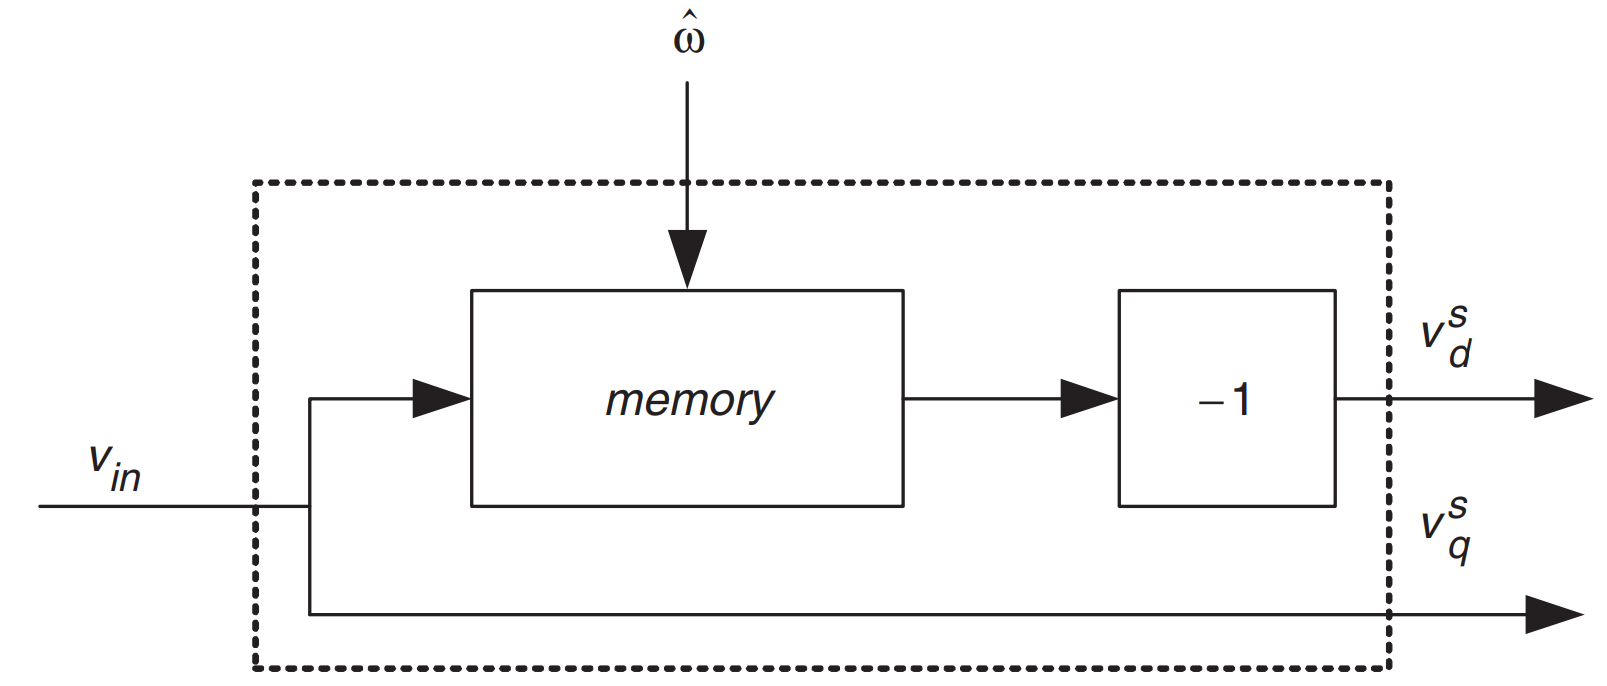
\includegraphics[width=.7\textwidth]{Fig. 4 Method using memory table.png}
					\caption{\centering \textit{4: Phương pháp sử dụng bảng bộ nhớ}}
					\label{fig:4: Phương pháp sử dụng bảng bộ nhớ}
				\end{figure}
					
	\end{frame}

% Slide 12
\begin{frame}[t]{(b) Phương pháp sử dụng góc pha và biên độ ước tính}	
	\begin{figure}[h]
		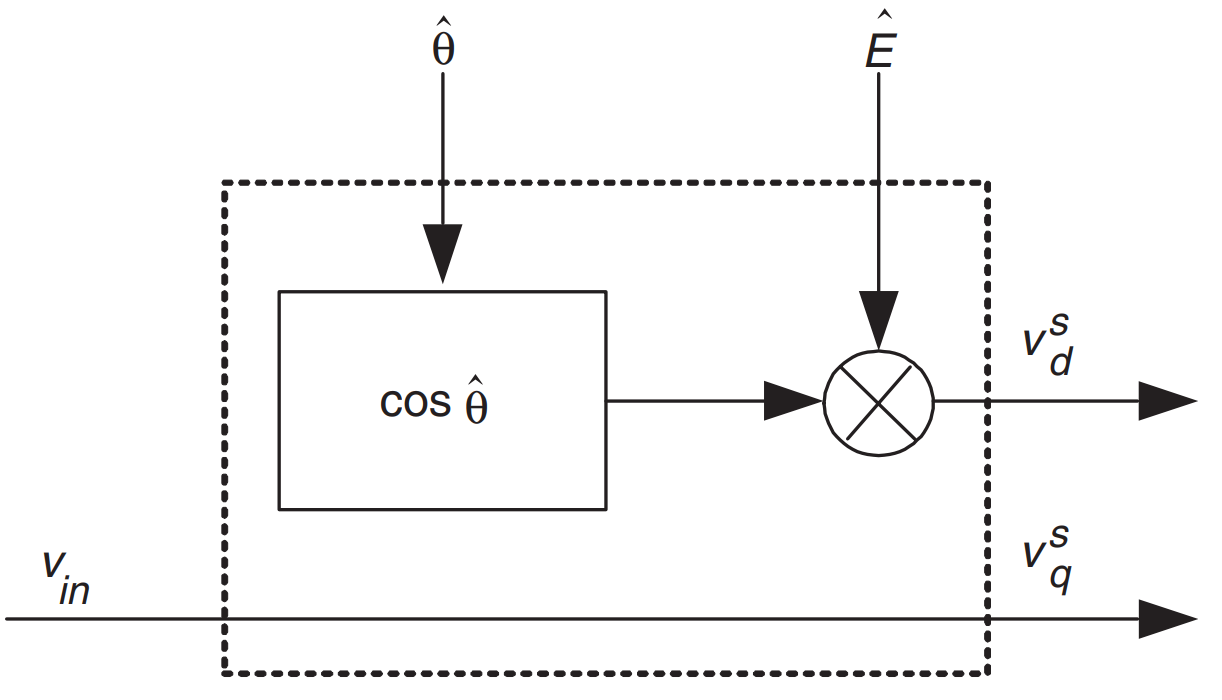
\includegraphics[width=.6\textwidth]{Fig. 5 Method using estimated phase angle and amplitude.PNG}
		\caption{\centering \textit{Phương pháp sử dụng góc pha và biên độ ước tính}}
		\label{fig:Phương pháp sử dụng góc pha và biên độ ước tính}
	\end{figure}
	Phương pháp này nhân biên độ ước lượng được $(\hat{E})$ với $\cos{\hat{\theta}}$ để thu được
	%$$v_d^s= \hat{E} \cos{\hat{\theta}} \cong E\cos{\theta} $$
	\begin{align*}
		v_d^s &= \hat{E} \cos{\hat{\theta}}\\
		{v}_q^s &=E\sin({\omega t})=v_{in}
	\end{align*}
	
\end{frame}

% Slide 13
\begin{frame}[t]{(c)  Phương pháp sử dụng bộ lọc bậc 2}
	
	$v_d^s$ và $v_q^s$ được tạo ra bằng cách cho $v_{in}$ đi qua bộ lọc thông thấp (LPF) bậc 2.
	
	 \begin{columns}
		\column{0.7\textwidth}
			\centering
			\begin{figure}[h]
				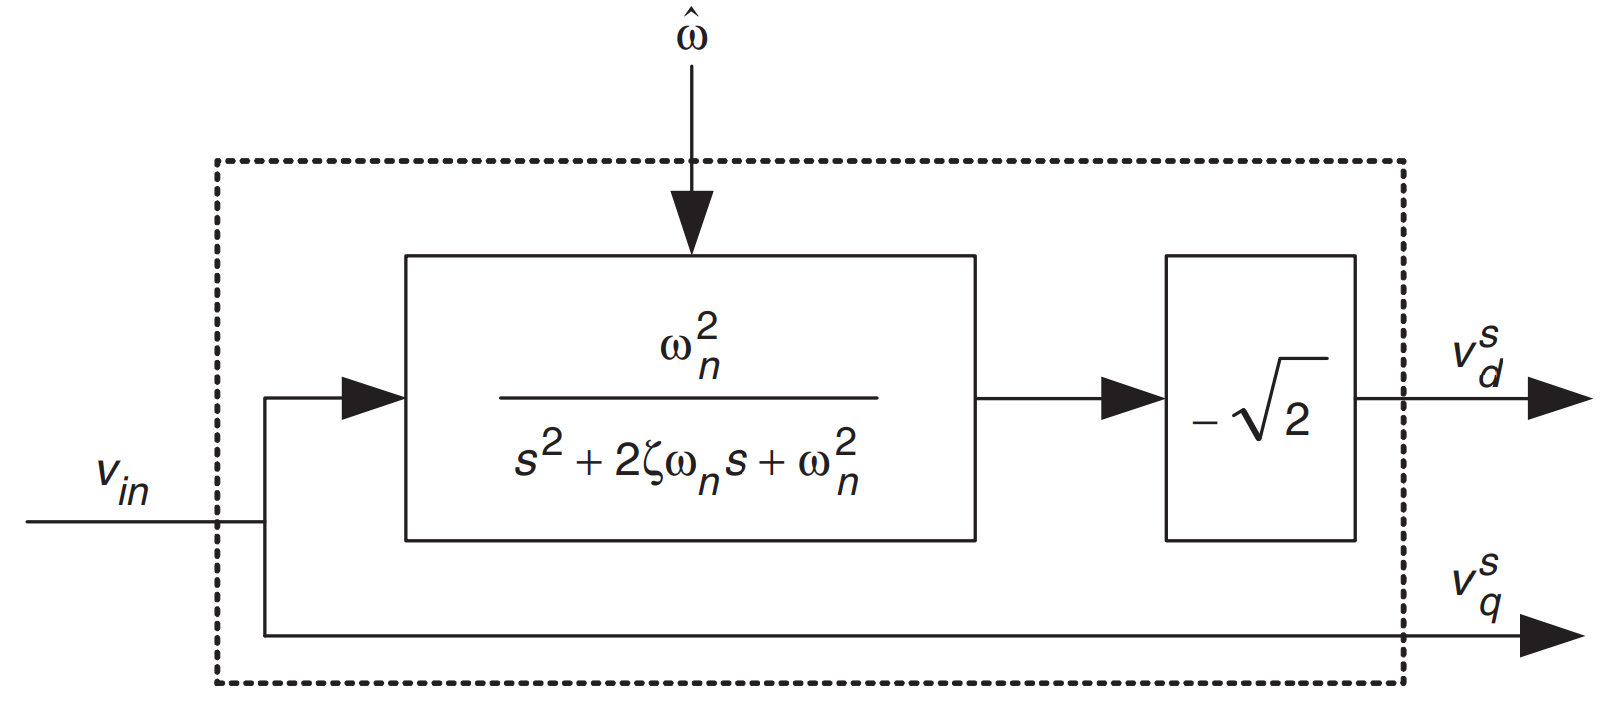
\includegraphics[width=1\textwidth]{Fig. 6 Method using second-order low-pass filter.PNG}
				\caption{\centering \textit{ Phương pháp sử dụng bộ lọc bậc 2}}
				\label{fig: Phương pháp sử dụng bộ lọc bậc 2}
			\end{figure}
		\column{0.3\textwidth}
			%\centering
			Hệ số giảm chấn $\zeta = \frac{1}{\sqrt{2}}$\\
			Tần số cộng hưởng ${\omega}_n = \hat{\omega} = \omega$
	\end{columns}
	
	
	Phương pháp này thu được
	$$v_d^s \cong {(-\sqrt{2}) \left( \frac{E}{\sqrt{2}} \sin{(\omega t - \frac{\pi}{2} )} \right) = E\cos{\omega t} }$$
	
\end{frame}

% Slide 14
	\begin{frame}[t]{(d) Phương pháp sử dụng bộ lọc bậc 1}
	
		Phương pháp này tạo ra $v_d^s$ và $v_q^s$ bằng cách cho $v_{in}$ đi qua bộ lọc thông thấp (LPF) bậc 1.	
		\begin{align*}
			v_d^s &= v_{in} - 2 \frac{E}{\sqrt{2}} \times \sin{(\omega t - \frac{\pi}{4} )} \\
			&=  E\sin({\omega t}) - 2 \frac{E}{\sqrt{2}} \times \sin{(\omega t - \frac{\pi}{4} )} = E\cos{(\omega t)} 
			%v_q^s &=E\cos({\omega t})
		\end{align*}
		\begin{figure}[h]
			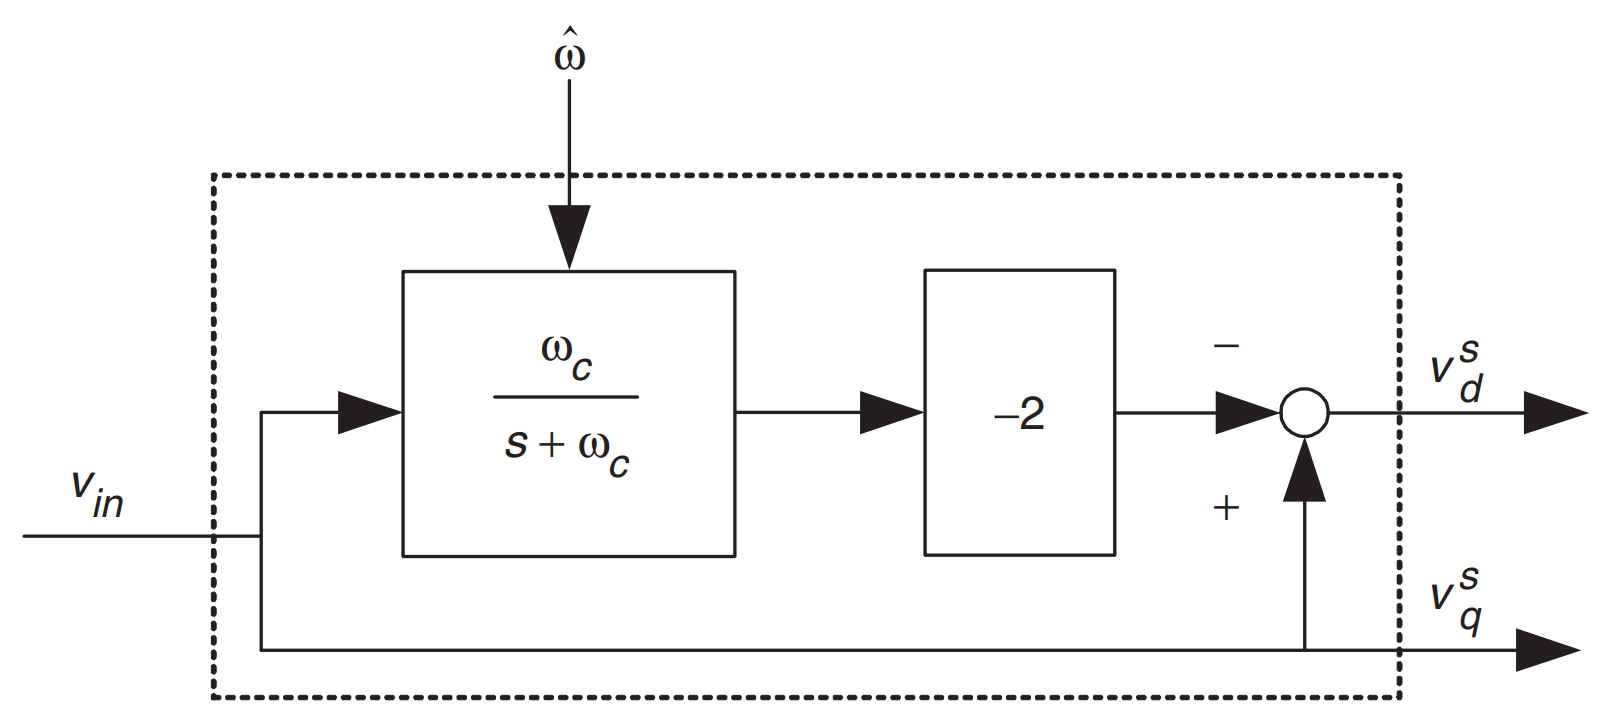
\includegraphics[width=.7\textwidth]{Fig. 7 Method using first-order low-pass filter.PNG}
			\caption{\centering \textit{Phương pháp sử dụng bộ lọc bậc 1}}
			\label{fig:Phương pháp sử dụng bộ lọc bậc 1}
		\end{figure}
	%$$v_d^s = v_{in} - {2 \frac{E}{\sqrt{2}} \times \sin{(\omega t - \frac{\pi}{4} )} = E\cos{\omega t} }$$
	
	\end{frame}

% Slide 15
\begin{frame}[t]{(e) Phương pháp sử dụng bộ lọc thông dải}
	
	Cho $v_{in}$ đi qua bộ lọc thông dải sẽ thu được $v_d^s$ và $v_q^s$.
	
		\begin{columns}
		\column{0.7\textwidth}
		\centering
			\begin{figure}[h]
				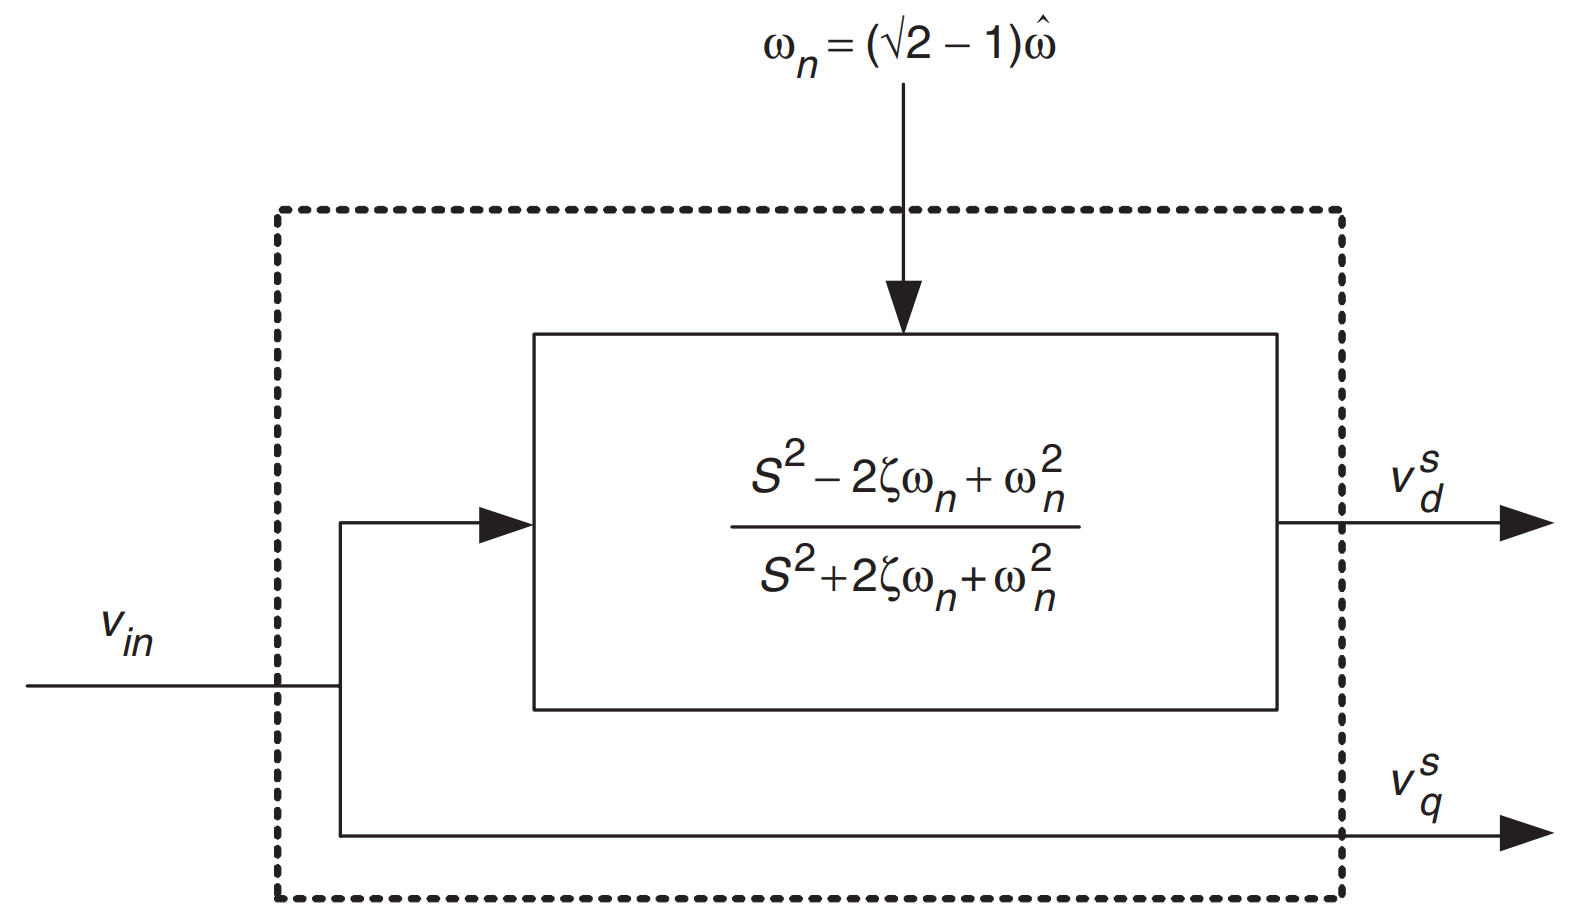
\includegraphics[width=1\textwidth]{Fig. 8 Method using all-pass filter.PNG}
				\caption{\centering \textit{Phương pháp sử dụng bộ lọc thông dải}}
				\label{fig:fig_8}
			\end{figure}
			\column{0.3\textwidth}
			%\centering
			Hệ số giảm chấn $\zeta = 1$\\
			Tần số cộng hưởng ${\omega}_n = (\sqrt{2} - 1)\hat{\omega}$\\
			và $\omega \cong \hat{\omega}$
		\end{columns}
		
		$$v_d^s = \hat{E} \cos{\hat{\theta}} \cong E\cos{\theta}$$
	
\end{frame}

%\subsection{3.2 Phase Controller}
% Slide 16
	\begin{frame}[t]{3.2 Bộ điều khiển pha}
		Trong hình dưới, bộ điều khiển pha tạo ra góc pha ước tính  $\hat{\theta}$, tần số ước tính $\hat{\omega}$ và biên độ ước tính $\hat{E}$ bằng cách sử dụng $v_d^s$ và $v_q^s$.		
		%\begin{figure}[h]	
			%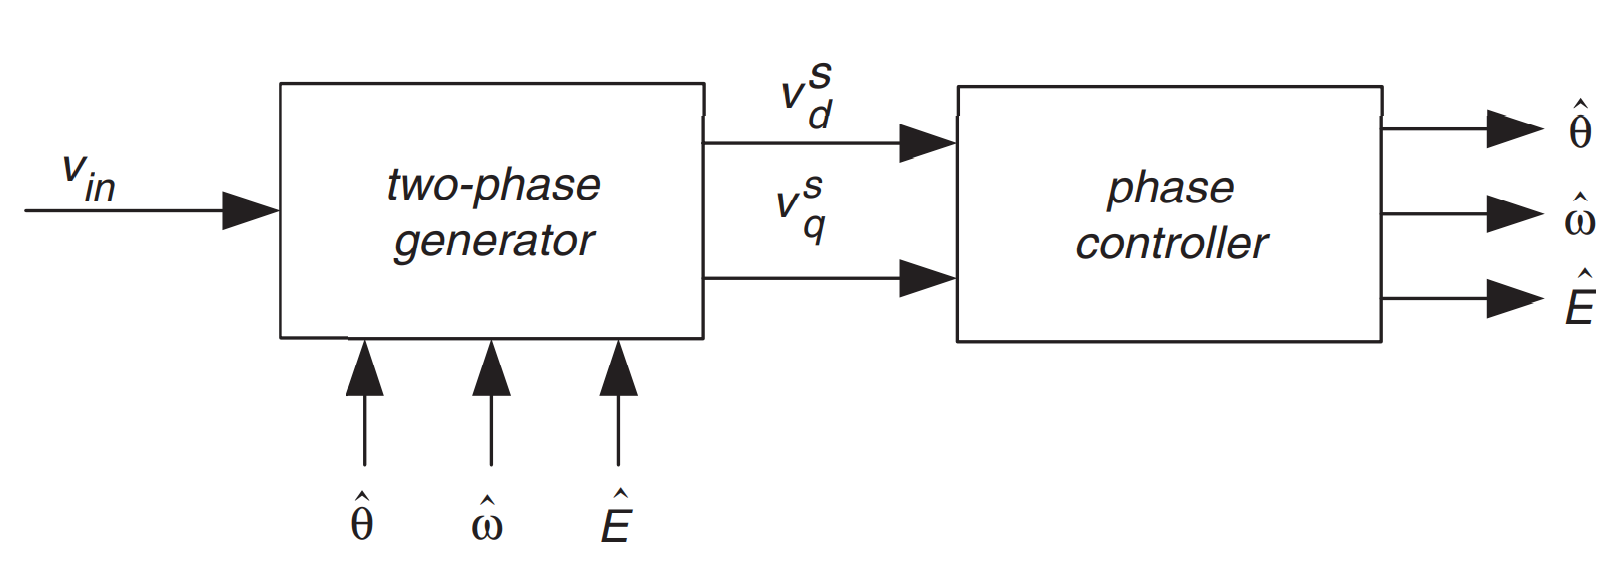
\includegraphics[width=1\textwidth]{Fig. 3 Virtual two-phase detector.PNG}

			%\label{fig:Virtual two-phase detector}
		%\end{figure}		
		\begin{enumerate}[(a)]
			\item Phương pháp sử dụng hàm arctan
			\item Phương pháp sử dụng khung đồng bộ
		\end{enumerate}
		%\begin{reusefigure}[ht]{fig:fig_8}
		%	\centering
		%	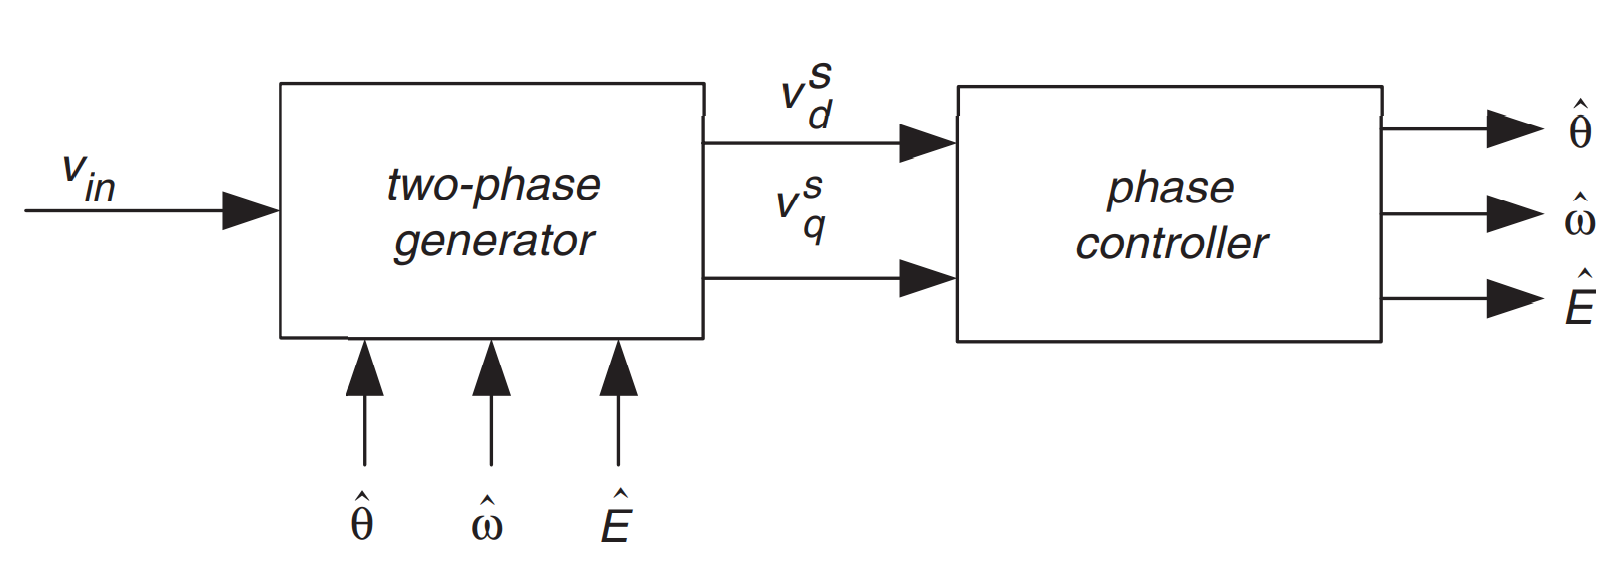
\includegraphics[height=3cm]{Fig. 3 Virtual two-phase detector.PNG}
		%	\caption{Bộ Dò 2 pha ảo}%\label{fig:caption-b}
		%\end{reusefigure}
		%\reusefigure[h]{fig:Bộ Dò 2 pha ảo}
		\begin{figure}[h]	
		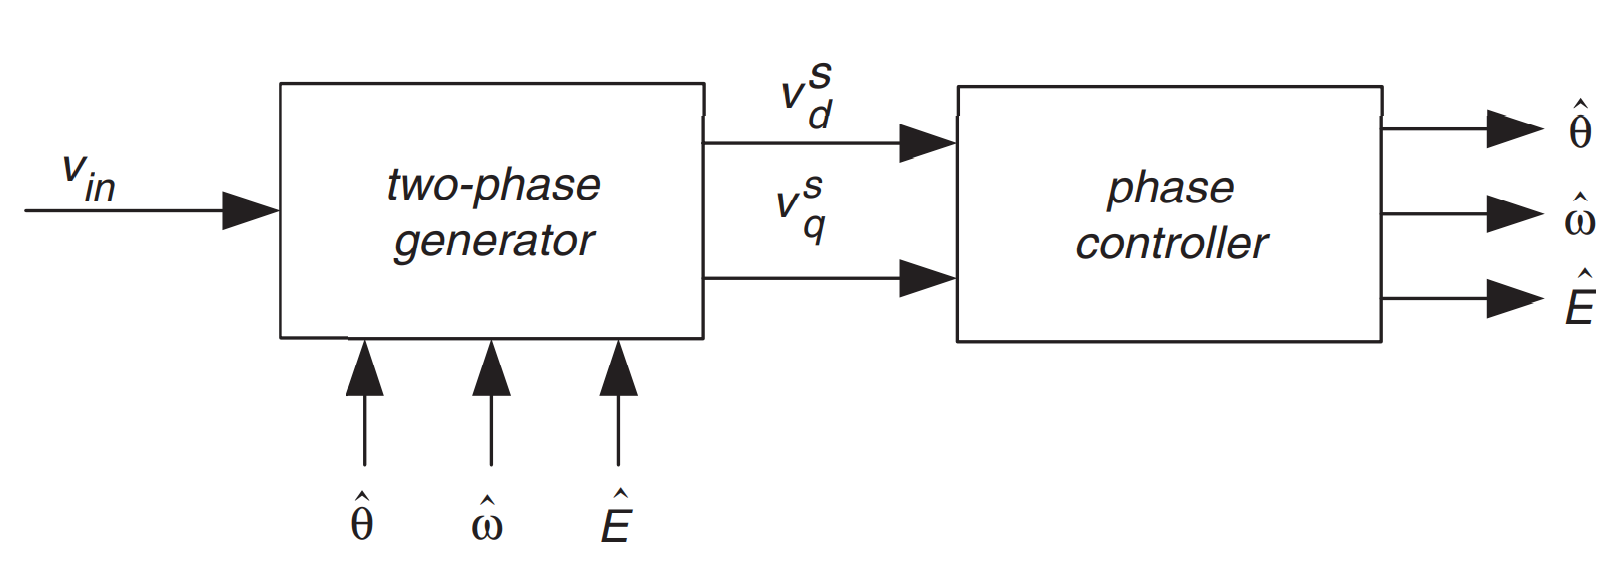
\includegraphics[width=1\textwidth]{Fig. 3 Virtual two-phase detector.PNG}
		
		\label{fig:Virtual two-phase detector}
		\end{figure}
	\end{frame}

% Slide 17
	\begin{frame}[t]{(a) Phương pháp sử dụng hàm arctan}
		\begin{figure}[h]
			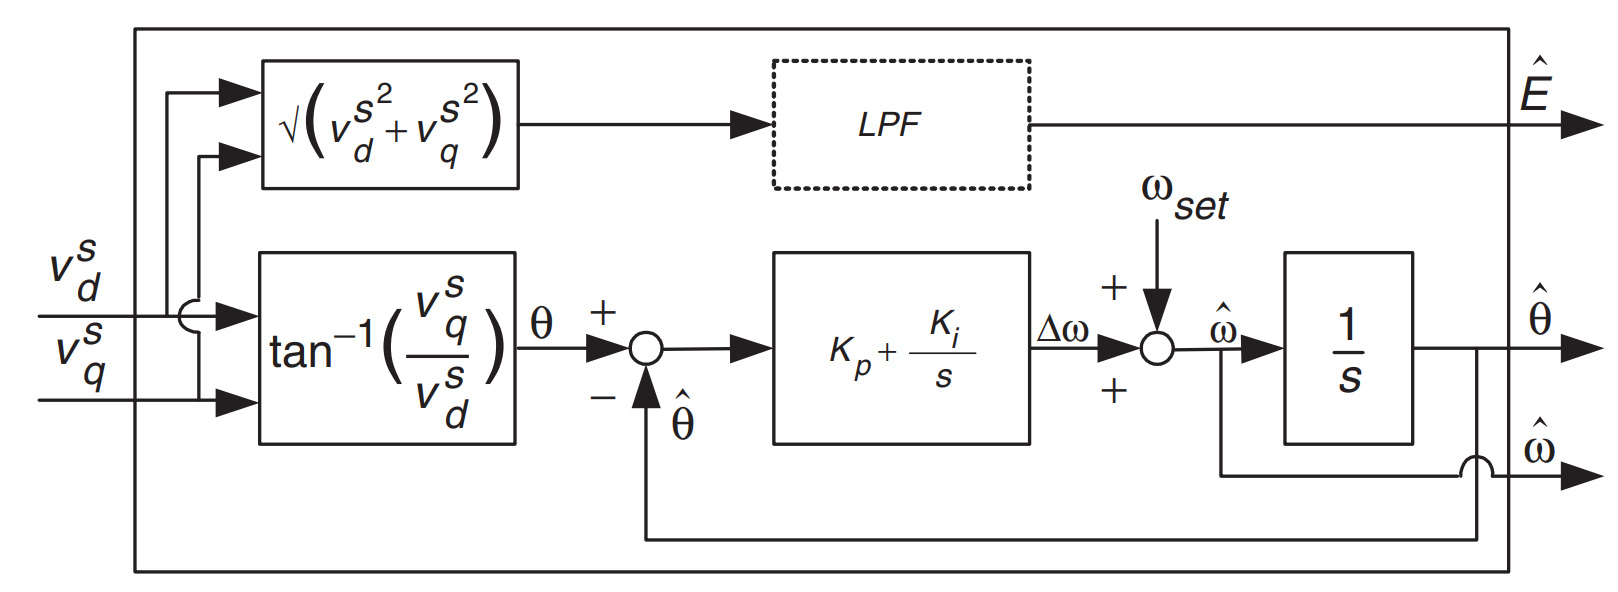
\includegraphics[width=1\textwidth]{Fig. 9 Method using arctangent function.PNG}
			\caption{\centering \textit{Phương pháp sử dụng hàm arctan}}\label{fig:Phương pháp sử dụng hàm arctan}
		\end{figure}
		\begin{align*}
			{\theta}^*&={\tan}^{-1} \left( {\frac{v_d^s}{v_q^s}} \right)\\
			\hat{E}&=\sqrt{{(v_d^s)^2}+{(v_q^s)^2}}
		\end{align*}
		%$${\theta}^*={\tan}^{-1} \left( {\frac{v_d^s}{v_q^s}} \right) $$
		%$$\hat{E}=\sqrt{{(v_d^s)^2}+{(v_q^s)^2}}$$
	
	\end{frame}

% Slide 18
	\begin{frame}[t]{(b) Phương pháp sử dụng khung đồng bộ}
		\begin{figure}[h]
			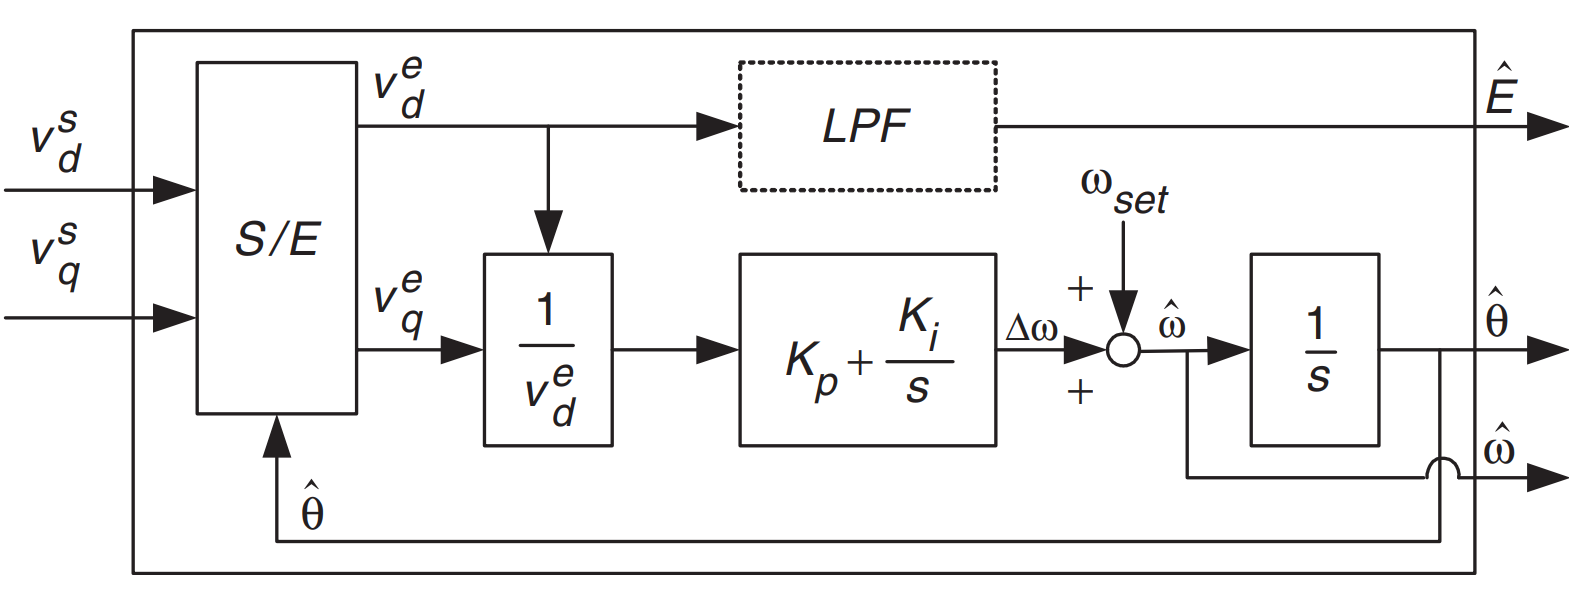
\includegraphics[width=.9\textwidth]{Fig. 10 Method using synchronous frame.PNG}
			\caption{\centering \textit{Phương pháp sử dụng khung đồng bộ}}
			\label{fig:Phương pháp sử dụng khung đồng bộ}
		\end{figure}
	
		\begin{columns}
			\column{0.5\textwidth}
				\centering
				\begin{align*}
					v_d^e &= v_d^s \cos{\hat{\theta}} + v_q^s \sin{\hat{\theta}}\\
					v_q^e &= -v_d^s \sin{\hat{\theta}} + v_q^s \cos{\hat{\theta}}
				\end{align*}
				%$v_d^e &= v_d^s \cos{\hat{\theta}} + v_q^s \sin{\hat{\theta}}$$
				%$$v_d^e &= -v_d^s \sin{\hat{\theta}} + v_q^s \cos{\hat{\theta}}$$
			\column{0.5\textwidth}
				\centering
				\begin{align*}
					v_d^e &= E \cos{\hat{\theta} - \theta} \cong E \\
					v_q^e &= E \sin{\theta - \hat{\theta}} \cong E(\theta - \hat{\theta})
				\end{align*}
				%$$v_d^e &= E \cos{\hat{\theta} - \theta} \cong E $$
			%	$$v_d^e &= E \sin{\theta - \hat{\theta}} \cong E(\theta - \hat{\theta})$$
			
		\end{columns}
		%$${\theta}^*={\tan}^{-1} \left( {\frac{v_d^s}{v_q^s}} \right) $$
		%$$\hat{E}=\sqrt{{(v_d^s)^2}+{(v_q^s)^2}}$$
		
	\end{frame}

%\subsection{3.3 Actual implementation}
% Slide 19
\begin{frame}[t]{3.3 Triển khai trong thực tế}
	\begin{figure}[h]
		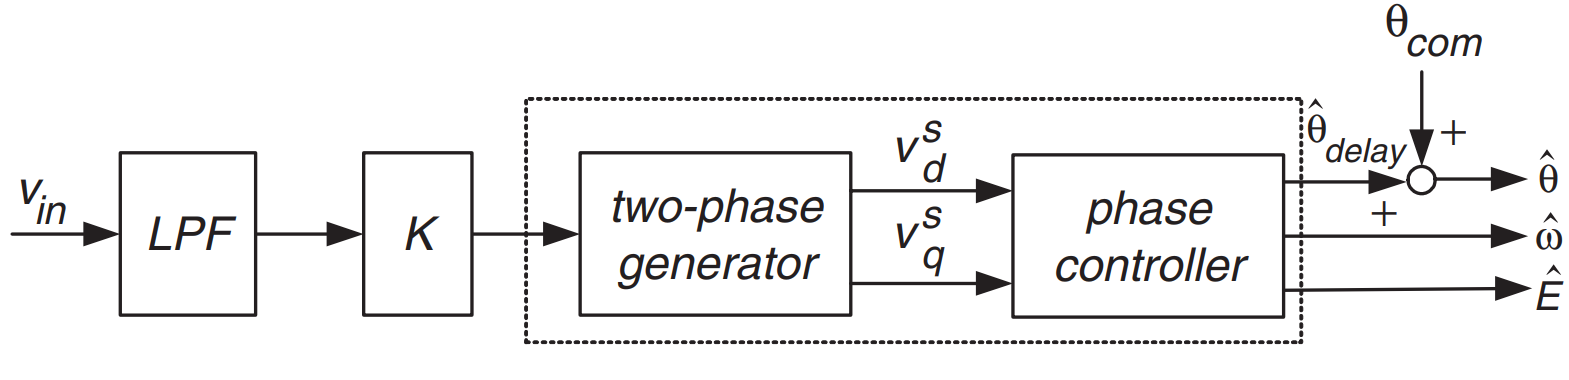
\includegraphics[width=1\textwidth]{Fig. 11 Overall configuration.PNG}
		\caption{\centering \textit{Cấu hình tổng thể}}
		\label{fig:Cấu hình tổng thể}
	\end{figure}
	Trong điều kiện thực tế, khi bộ lọc được đưa vào để giảm nhiễu, người ta sẽ thêm khâu khuếch đại với HSKĐ $K$; góc bù $\theta_{com}$ được thêm vào để bù trễ pha da LPF gây ra.\\Hàm truyền của LPF là F(s) thì
	\begin{columns}
		\column{0.5\textwidth}
		\centering
		\begin{align*}
			K = \frac{1}{|F(j \hat{\theta})|}\\
			%v_d^e &= -v_d^s \sin{\hat{\theta}} + v_q^s \cos{\hat{\theta}}
		\end{align*}

		\column{0.5\textwidth}
		\centering
		\begin{align*}
			{\theta}_{com} = {|F(j \hat{\theta})|} \\
			%v_d^e &= E \sin{\theta - \hat{\theta}} \cong E(\theta - \hat{\theta})
		\end{align*}
		
	\end{columns}
	
\end{frame}




\section{4 Thực nghiệm}
% Slide 20
	\begin{frame}[t]{4 Thực nghiệm}
		Các thí nghiệm đã được thực hiện để đánh giá mọi phương pháp liên quan đến đáp ứng động, phản hồi trạng thái ổn định, đáp ứng với sự sụt giảm điện áp và phản ứng với sự xuất hiện sóng hài (bậc ba và bậc năm).
		
		Trong các thí nghiệm, biên độ của điện áp đầu vào là 220V RMS, tần số là 60 Hz và biên độ đỉnh của sóng hài đưa vào là 30V với tần số là 1kHz. Bộ điều khiển bắt đầu khi góc pha của điện áp đầu vào là $\pi$.
		
		Khi bơm lên một thành phần sóng hài, biên độ của điện áp đầu vào là 220V RMS, tần số là 60 Hz và các thành phần sóng hài bậc ba và thứ năm được đưa vào.
		
		Phương trình sau đây được đưa ra sử dụng biên độ ước tính $\hat{E}$ và góc pha ước tính $\hat{\theta}$:	
		$\hat{v}_{in} = \hat{E}\sin{\hat{\theta}} $
		
	\end{frame}

% Slide 21
\begin{frame}[t]{4 Thực nghiệm}
	\begin{table}
		%\caption{\label{tab:table-1}Sự kết hợp của bộ tạo 2 pha và bộ điều khiển pha.}
		\begin{tabular}{lll}
			\toprule
			PP & Bộ tạo hai pha ảo & Bộ điều khiển pha   \\
			\midrule
			1	& PPSD bảng bộ nhớ		& PPSD hàm arctan \\
			2	& PPSD góc pha và biên độ ước tính  & PPSD hàm arctan  \\
			3   & PPSD bộ lọc bậc 2 & PPSD hàm arctan  \\
			4	& PPSD bộ lọc bậc 1  & PPSD hàm arctan \\
			5	& PPSD bộ lọc bậc thông dải  & PPSD hàm arctan \\
			6	& PPSD bảng bộ nhớ  & PPSD khung đồng bộ \\
			7	& PSD góc pha và biên độ ước tính  & PPSD khung đồng bộ \\
			8	& PPSD bộ lọc bậc 2  & PPSD khung đồng bộ \\
			9	& PPSD bộ lọc bậc 1  & PPSD khung đồng bộ \\
			10	& PPSD bộ lọc bậc thông dải  & PPSD khung đồng bộ \\
			\bottomrule
			%\caption{\label{tab:table-1}Sự kết hợp của bộ tạo 2 pha và bộ điều khiển pha.}
		\end{tabular}
		\caption{\label{tab:table-1}Sự kết hợp của bộ tạo 2 pha và bộ điều khiển pha.}
	\end{table}	
	
\end{frame}


% Slide 22
\begin{frame}[t]{4.1 Đáp ứng động}
	  \begin{figure}
		\begin{subfigure}{0.5\textwidth}
			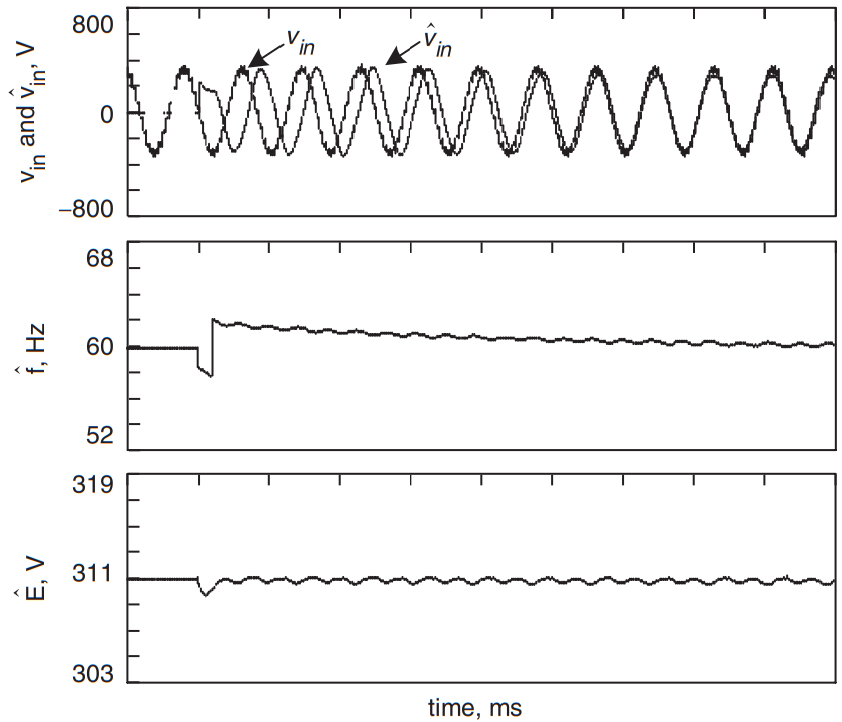
\includegraphics[width=\linewidth]{fig12a}
			\caption{Phương pháp 1}
		\end{subfigure}%                                                                                                                          
		\begin{subfigure}{0.5\textwidth}
			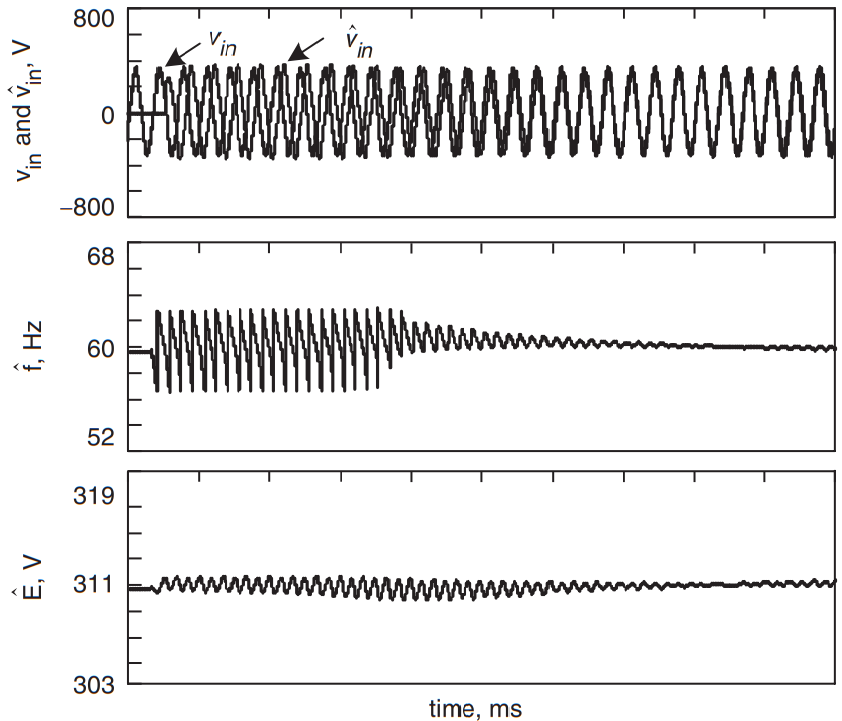
\includegraphics[width=\linewidth]{fig12b}
			\caption{Phương pháp 2}
		\end{subfigure}
		\caption{Các đặc điểm ước tính khi khởi động}
	\end{figure}	
	
\end{frame}

% Slide 23
\begin{frame}[t]{4.1 Đáp ứng động}
	\begin{figure}
		\ContinuedFloat
		\begin{subfigure}{0.5\textwidth}
			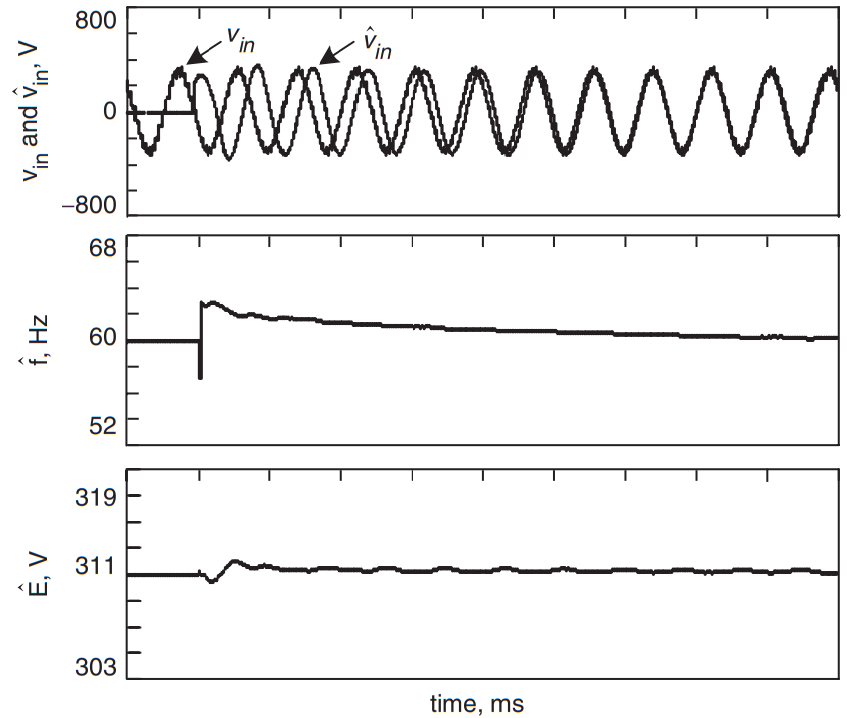
\includegraphics[width=\linewidth]{fig12c}
			\caption{Phương pháp 3}
		\end{subfigure}%                                                                                                                          
		\begin{subfigure}{0.5\textwidth}
			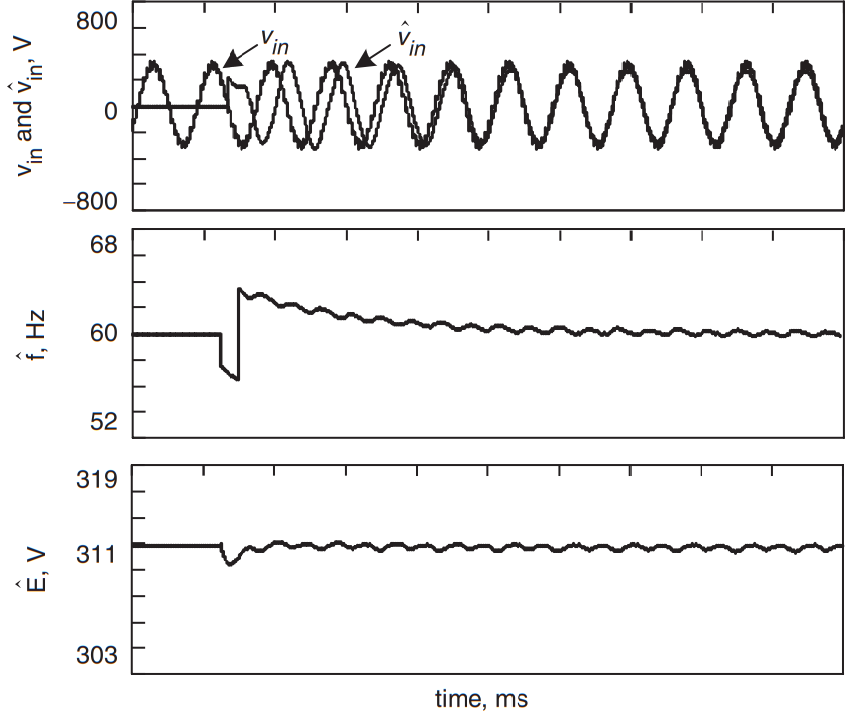
\includegraphics[width=\linewidth]{fig12d}
			\caption{Phương pháp 4}
		\end{subfigure}
		\caption{Các đặc điểm ước tính khi khởi động}
	\end{figure}	
	
\end{frame}

% Slide 24
\begin{frame}[t]{4.1 Đáp ứng động}
	\begin{figure}
		\ContinuedFloat
		\begin{subfigure}{0.5\textwidth}
			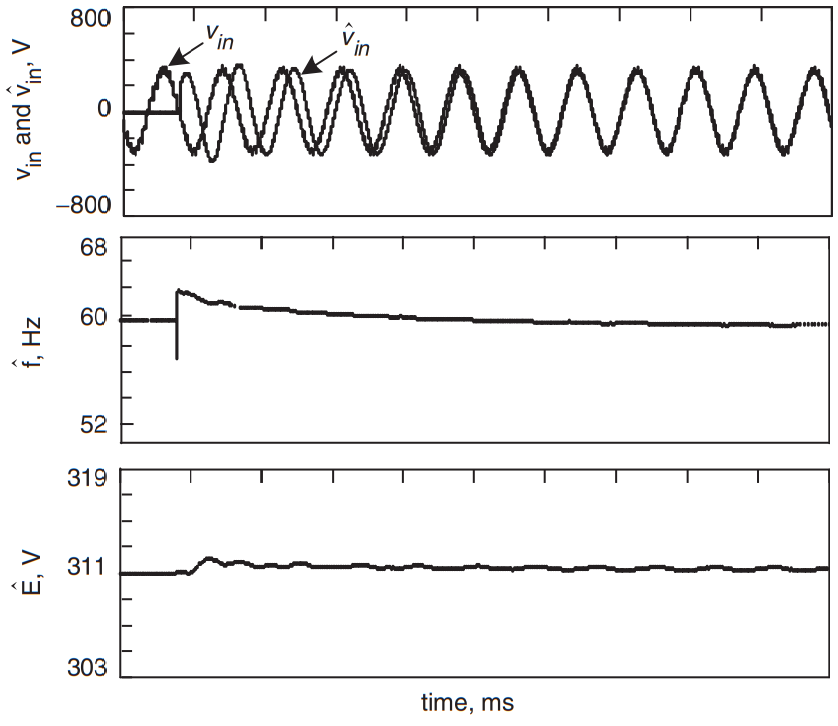
\includegraphics[width=\linewidth]{fig12e}
			\caption{Phương pháp 5}
		\end{subfigure}%                                                                                                                          
		\begin{subfigure}{0.5\textwidth}
			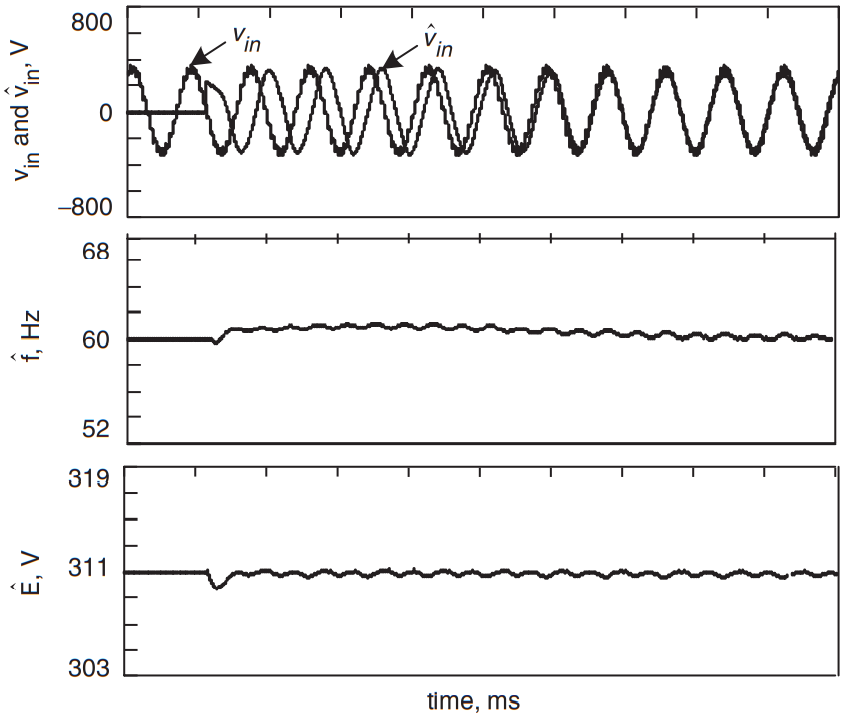
\includegraphics[width=\linewidth]{fig12f}
			\caption{Phương pháp 6}
		\end{subfigure}
		\caption{Các đặc điểm ước tính khi khởi động}
	\end{figure}	
	
\end{frame}

% Slide 25
\begin{frame}[t]{4.1 Đáp ứng động}
	\begin{figure}
		\ContinuedFloat
		\begin{subfigure}{0.5\textwidth}
			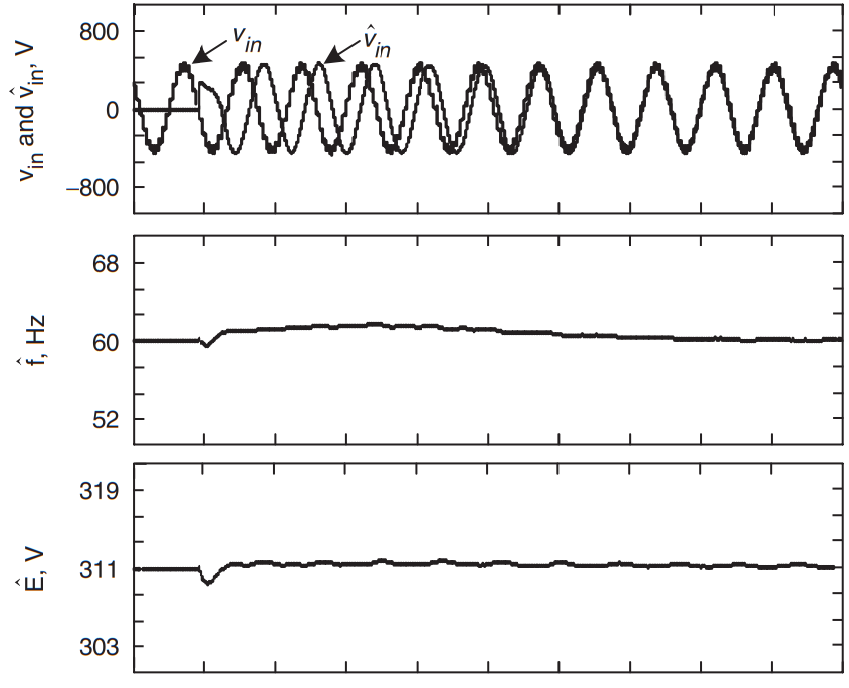
\includegraphics[width=\linewidth]{fig12h}
			\caption{Phương pháp 7}
		\end{subfigure}%                                                                                                                          
		\begin{subfigure}{0.5\textwidth}
			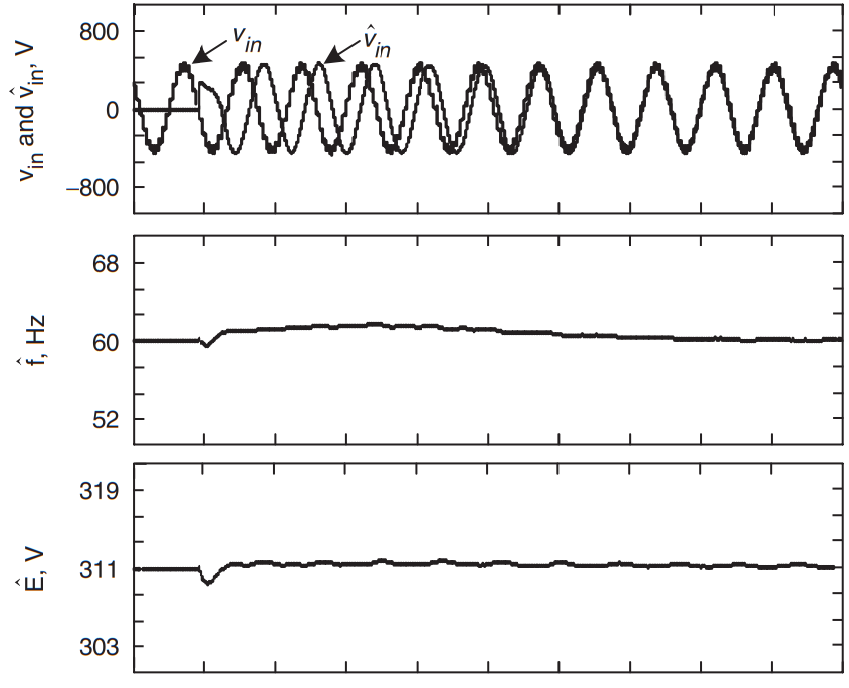
\includegraphics[width=\linewidth]{fig12h}
			\caption{Phương pháp 8}
		\end{subfigure}
		\caption{Các đặc điểm ước tính khi khởi động}
	\end{figure}	
	
\end{frame}

% Slide 26
\begin{frame}[t]{4.1 Đáp ứng động}
	\begin{figure}
		\ContinuedFloat
		\begin{subfigure}{0.5\textwidth}
			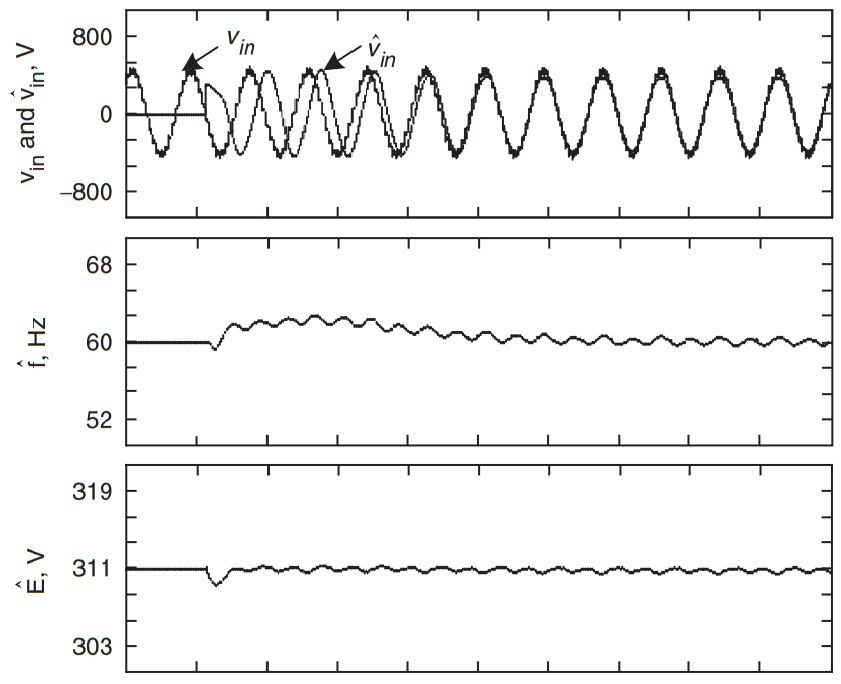
\includegraphics[width=\linewidth]{fig12i}
			\caption{Phương pháp 9}
		\end{subfigure}%                                                                                                                          
		\begin{subfigure}{0.5\textwidth}
			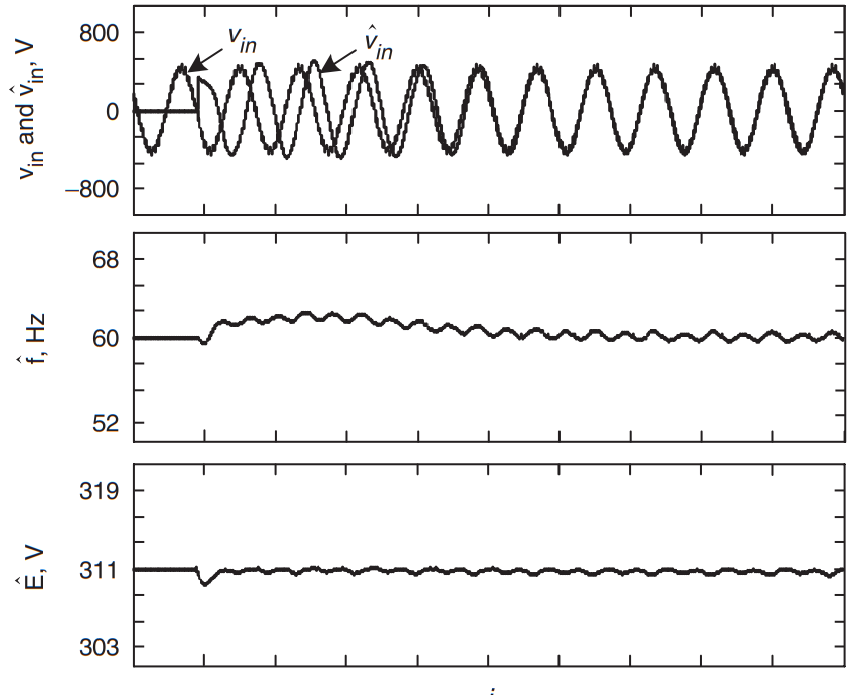
\includegraphics[width=\linewidth]{fig12j}
			\caption{Phương pháp 10}
		\end{subfigure}
		\caption{Các đặc điểm ước tính khi khởi động}
	\end{figure}	
	
\end{frame}

% Slide 27
\begin{frame}[t]{4.1 Đáp ứng động}
	\justifying
	\begin{table}
	%	\centering
		\begin{tabular}{lllllllllll}
			\toprule
			Method & 1 	& 2		&3&4&5&6&7&8&9&10   \\
			\midrule
			Time   & 120 	& 300  &140&100&100&120&250&120&100&100\\
			\bottomrule
		\end{tabular}
		\caption{\label{tab:table-1}So sánh thời gian ước tính.}
	\end{table}
	
\end{frame}

% Slide 28
\begin{frame}[t]{4.1 Đáp ứng động}
	
	Hình 12 cho thấy phản ứng động của các phương pháp được đề xuất. 
	
	Góc pha ước tính, biên độ và tần số đều được đồng bộ hóa với giá trị của điện áp đầu vào trong khoảng từ 100 ms đến 300 ms, như thể hiện trong Bảng 2.
	
	Các phương pháp sử dụng góc pha và biên độ ước tính (2 và 7) rất dễ thực hiện, nhưng chúng có đặc tính đáp ứng động rất kém. 
	
	Góc pha đồng bộ ở 250–300 ms đối với phương pháp 2 và 7, trong khi các phương pháp khác đồng bộ ở 100–140 ms. 
	
	Các phương pháp sử dụng bảng bộ nhớ (1 và 6) cho thấy hiệu suất vừa phải, nhưng chúng gặp khó khăn khi triển khai yêu cầu kích thước bộ nhớ lớn. 
	
	
\end{frame}	

% Slide 29
\begin{frame}[t]{4.1 Đáp ứng động}
	
	Các phương pháp sử dụng bộ lọc tương đối dễ thực hiện và chúng có hiệu suất tốt. 
	
	Các phương pháp sử dụng bộ lọc thông thấp bậc nhất (4 và 9) và bộ lọc thông thấp (5 và 10) cho thấy thời gian ước tính ngắn nhất và các phương pháp sử dụng bộ lọc thông thấp bậc hai (3 và 8) cho thấy ít dao động hơn. 
	
	Các phương pháp sử dụng Hàm arctangent (1–5) rất dễ hiểu nhưng gặp khó khăn khi thực hiện trong việc tính toán hàm arctangent. 
	
	Các phương pháp sử dụng khung đồng bộ (6–10) ưu việt hơn các phương pháp sử dụng hàm arctangent trong việc thực hiện. 
	
	Hơn nữa, trong thử nghiệm này, chúng cho thấy hiệu suất tốt hơn một chút so với các phương pháp sử dụng hàm arctangent. 
	
	
\end{frame}


% Slide 30
\begin{frame}[t]{4.2 Phản hồi ở trạng thái ổn định}
	
	Hình 13 cho thấy đáp ứng trạng thái ổn định cho phương pháp sử dụng bộ lọc bậc hai cho bộ phát hai pha và khung đồng bộ cho pha. 
	Bất chấp nhiễu, biên độ và góc pha của điện áp đầu vào ước tính đã được đồng bộ hóa thành công với điện áp đầu vào.
	 
	Trong khi đó, với các phương pháp khác, điện áp đầu vào ước tính đã bám theo điện áp đầu vào thực, cho kết quả tương tự. 

	\begin{figure}[h]
	%\label{fig:Zero-cross-detection method}
	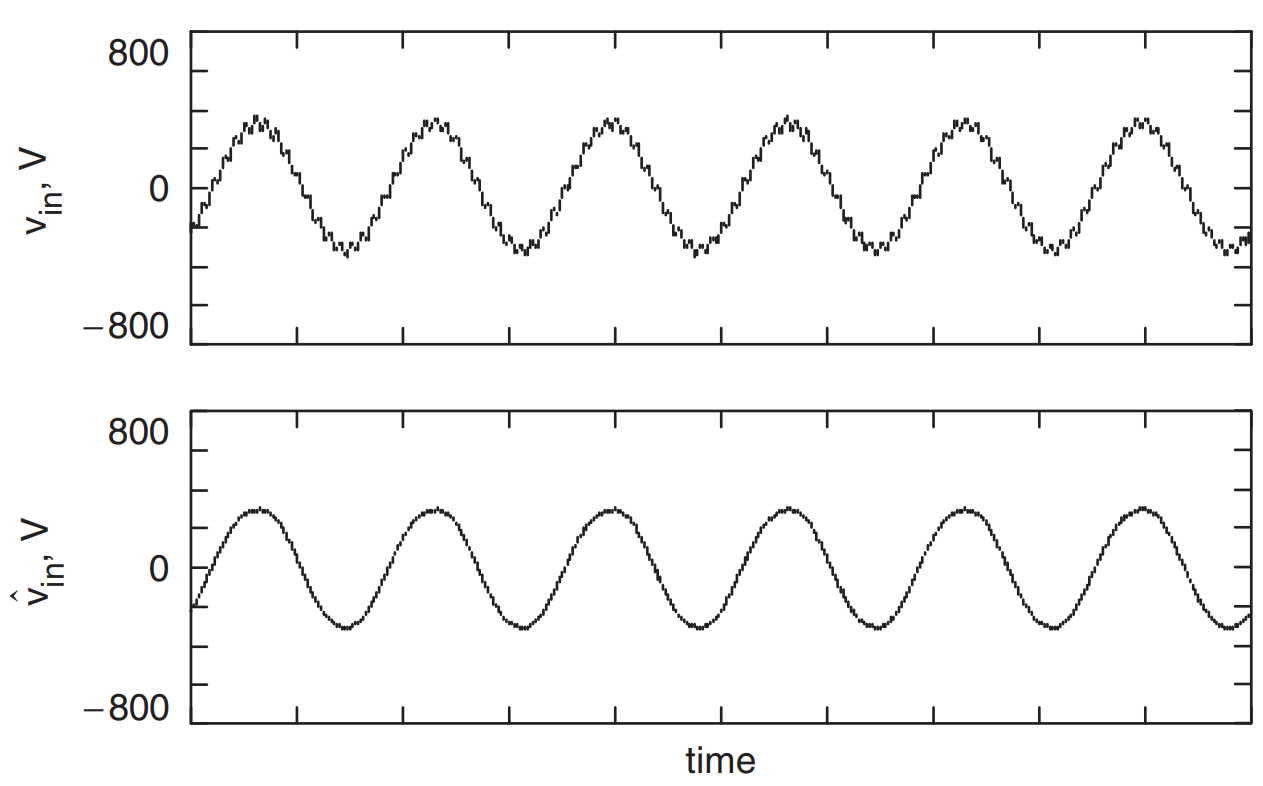
\includegraphics[width=0.5\textwidth]{Fig. 13 Estimated characteristics under steady state.PNG}  
	\caption{\textit{Đặc tính ước tính ở trạng thái ổn định}}
	\end{figure}
\end{frame}

% Slide 31
\begin{frame}[t]{4.3 Đáp ứng với độ sụt giảm điện áp}
	%
	%Hình 14 cho thấy đáp ứng với sự sụt giảm điện áp 50$\%$ khi sử dụng bộ lọc bậc hai cho máy phát hai pha và khung đồng bộ cho bộ điều khiển pha. 
	%
	%Theo tiêu chuẩn IEEE 929: 2000, điều kiện hoạt động bình thường cho các hệ thống PV nhỏ là 88–110$\%$ điện áp danh định, tức là cường độ 274–342V.
	%
	\begin{columns}
		\column{0.5\textwidth}
			\justifying
			Hình 14 cho thấy đáp ứng với sự sụt giảm điện áp 50$\%$ khi sử dụng bộ lọc bậc hai cho máy phát hai pha và khung đồng bộ cho bộ điều khiển pha.\\[8pt]
			Theo tiêu chuẩn IEEE 929: 2000, điều kiện hoạt động bình thường cho các hệ thống PV nhỏ là 88–110$\%$ điện áp danh định, tức là cường độ 274–342V.
		\column{0.5\textwidth}
		\centering
			\begin{figure}[h]
				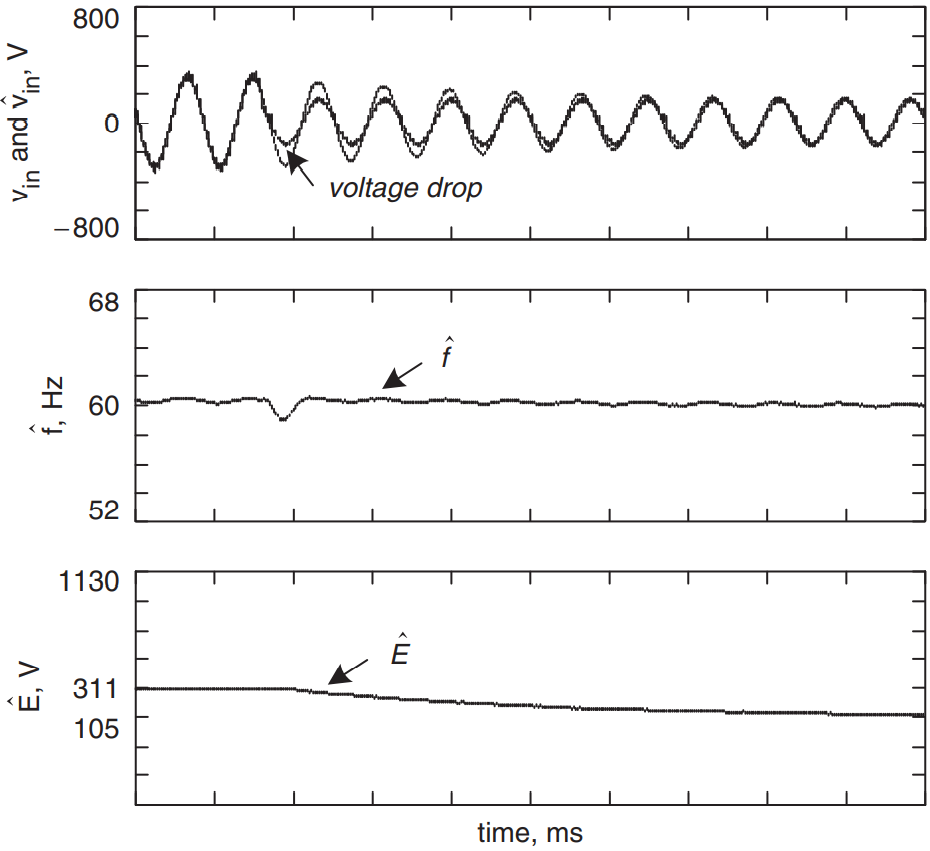
\includegraphics[width=1\textwidth]{Fig. 14 Estimation characteristics with voltage drop.PNG}
				\caption{\centering \textit{Đặc tính ước tính với sự sụt giảm điện áp}}
				%\label{fig:Method using all-pass filter}
			\end{figure}
	\end{columns}
	
\end{frame}

% Slide 32
\begin{frame}[t]{4.4 Đáp ứng với thành phần sóng hài được thêm vào}
	\begin{figure}
		\begin{subfigure}{0.5\textwidth}
			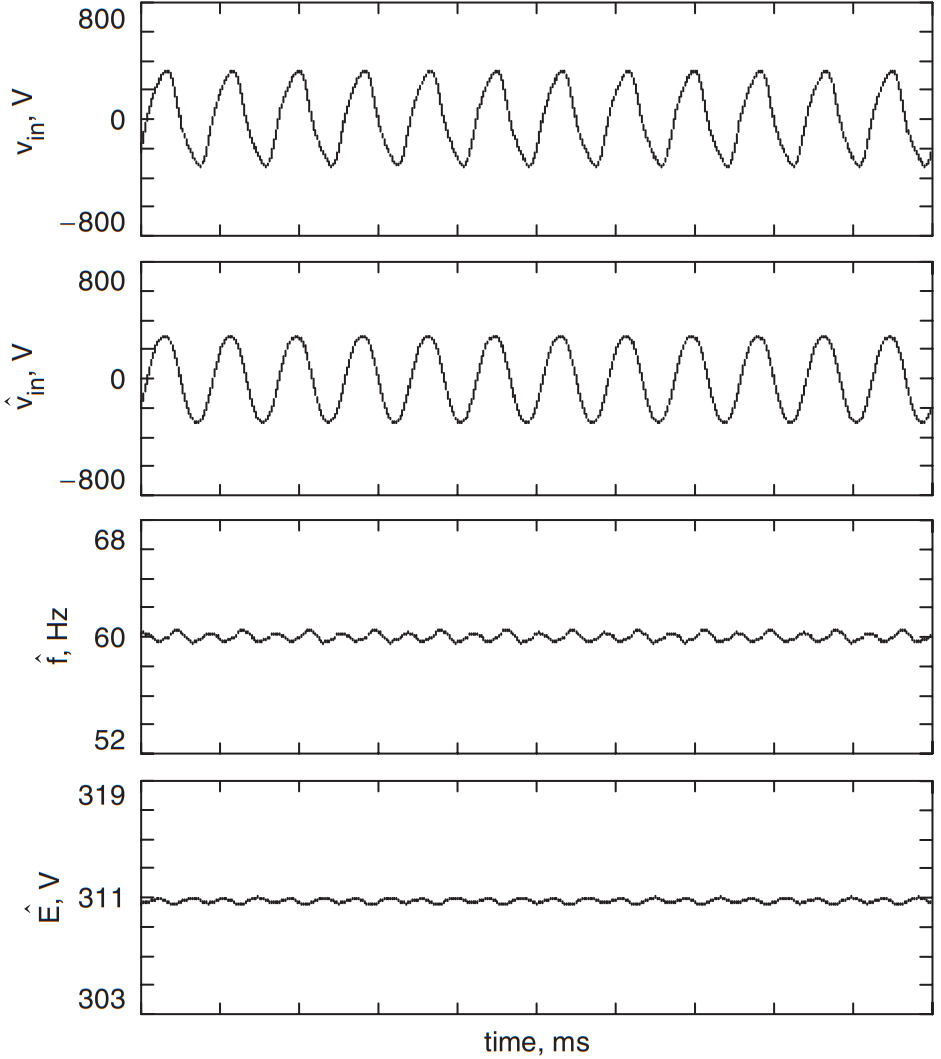
\includegraphics[width=0.9\linewidth]{fig15a}
			\caption{Tác động sóng hài bậc 3} %\label{fig:1a}
		\end{subfigure}%
		\hspace*{\fill}   % maximize separation between the subfigures
		\begin{subfigure}{0.5\textwidth}
			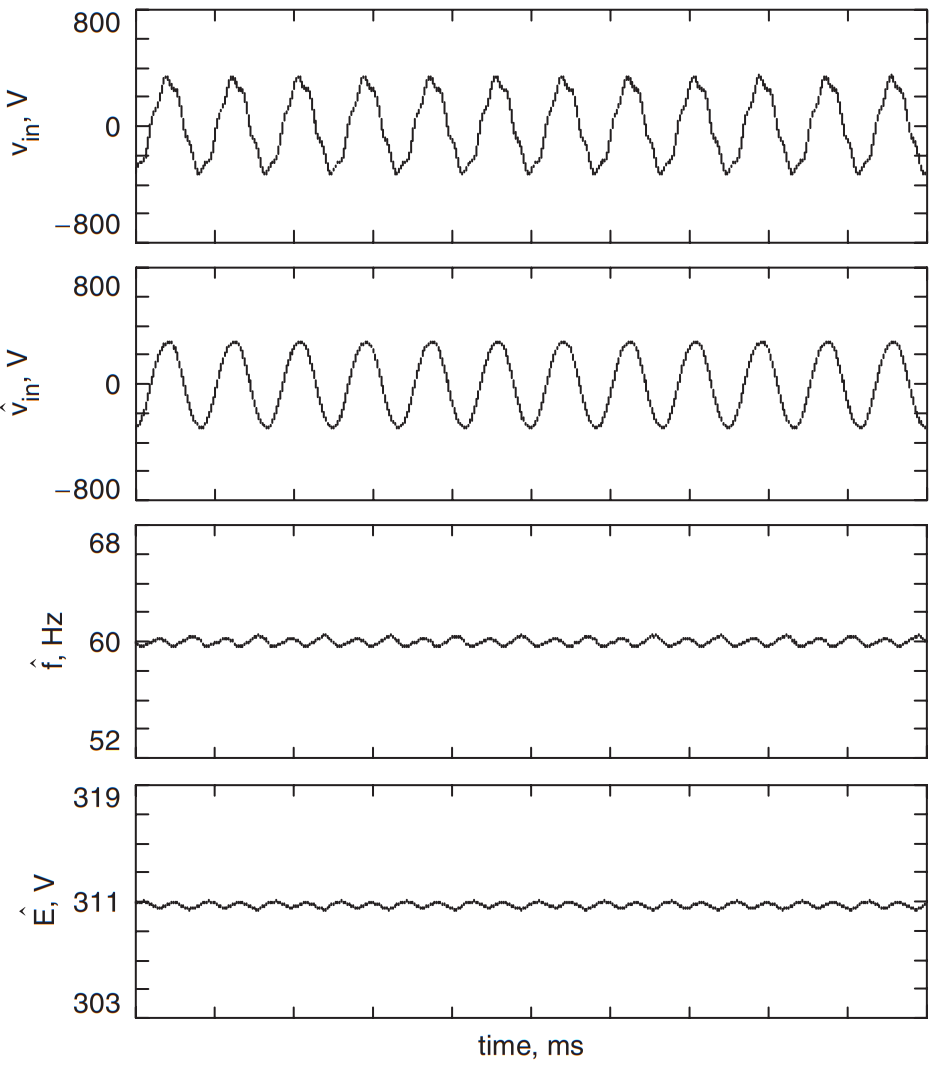
\includegraphics[width=0.9\linewidth]{fig15b}
			\caption{Tác động sóng hài bậc 5} %\label{fig:1b}
		\end{subfigure}%
		
		\caption{Đặc tính ước tính với sóng hài bậc 3 và bậc 5} %\label{fig:1}
	\end{figure}
	
\end{frame}

% Slide 33
\begin{frame}[t]{4.4 Đáp ứng với thành phần sóng hài được thêm vào}
	
	Hình 15 cho thấy đáp ứng với thành phần sóng hài được đưa vào (bậc 3 và bậc 5) khi sử dụng bộ lọc bậc hai cho bộ phát hai pha và khung đồng bộ cho bộ điều khiển pha. 
	
	Trong khi đó, với các phương pháp khác, điện áp đầu vào ước tính đã bám theo điện áp đầu vào thực, cho kết quả tương tự.
	
\end{frame}

 

\section{5 Kết luận}
% Slide 34
\begin{frame}[t]{5 Kết luận}
	
	Ta biết thêm một cách tiếp cận mới để điều khiển PLL kỹ thuật số bằng cách sử dụng bộ dò 2 pha ảo đã được đề xuất và xác minh bằng các thí nghiệm.
	
	Bộ dò hai pha ảo bao gồm một bộ tạo hai pha và bộ điều khiển pha, hai pha có năm tùy chọn, trong khi bộ điều khiển pha có hai tùy chọn.
	
	Do đó, khi máy tạo hai pha được kết hợp với bộ điều khiển pha, điều này cung cấp mười phương pháp kỹ thuật số-PLL.
	Kết quả thực nghiệm đã chứng minh rằng các phương pháp sử dụng bảng bộ nhớ và bộ lọc là vượt trội hơn hẳn. 
	
	Tuy nhiên, do khó triển khai với các phương pháp sử dụng bảng bộ nhớ, các phương pháp sử dụng bộ lọc và khung đồng bộ được cho là thích hợp hơn.	
	
\end{frame}

%Silde 34
\begin{frame}[standout]
	\flushleft
	\Huge
	Thanks for watching!
\end{frame}

	
\end{document}
